\documentclass{article}
\usepackage[T1]{fontenc}
\usepackage[utf8]{inputenc}
\usepackage[icelandic]{babel}
\usepackage{graphicx}
\usepackage{fancyhdr}
\usepackage{listings}
\usepackage{xcolor}
\usepackage{lipsum}
\usepackage{hyperref}
\pagestyle{fancy}
\fancyhf{}
\rhead{Vélmenni II}
\lhead{\begin{picture}(0,0) \put(0,0){\includegraphics[width=3cm]{img/tskoli}} \end{picture}}
\lfoot{Ótitlað RetroPi verkefni}
\rfoot{\thepage}
\begin{document}
\title{Vélmenni II}
\author{Guðni Natan Gunnarsson}
\maketitle
\begin{figure}[h]
\centering
\includegraphics[scale=.65]{img/tskoli}
\includegraphics[scale=1]{img/rob2b3u_img}
\end{figure}
\newpage
\tableofcontents
\newpage
\section{Inngangur}
Hér skal gera lýsingu á verkefninu þ.e hvað,  hvernig og  hvaða forritunarmál, fyrir hverja og hvaða notagildi verkefnið hefur. Minnst 500 orð. Notagildi skiptir miklumáli, reynið að sjá fyrir ykkur hverjir geti notað vélmennið ykkar og í hvaða tilgangi.  Þá kemur í ljós að 500 orð er frekar lítið :-) Hér er gott að byrja á því að lesa til um Arduino en allt hjá þeim er open-sourse og svo er hægt að lesa sér til um efnið í útgefnum bókum sem "programming Arduino \cite{monk} Skoðið vel heimildaskrá og skránna mybib.bib. Hér er gott að lýsa högun kerfisins með orðum og mynd sem þið getið gert í draw.io sjá mynd: Ég er bara að prófa að setja inn smá auka texta.
\begin{figure}[h]
\includegraphics[scale=.3]{img/system}
\end{figure}

\section{Vélbúnaður}
Hér skal gera töflu eða lista yfir allan búnað sem notaður er gott væri að þið nýttuð ykkur töfluna hér fyrir neðan:


\begin{tabular}{l c c l}
    \textbf{Nafn} & \textbf{Hlekkur} & \textbf{Útvegað} & \textbf{Verð} \\
    \hline
    Raspberry Pi 3 B & \href{https://www.adafruit.com/products/3055}{Adafruit} & $\surd $& \$39.95\\
    \hline
    7'' Display & \href{https://www.adafruit.com/products/2354}{Adafruit} & & \$47.50\\
    \hline
    PowerBoost 1000 & \href{https://www.adafruit.com/products/2465}{Adafruit} & & \$19.95 \\
    \hline
    SNES Controller & \href{https://www.adafruit.com/products/131}{Adafruit} & & \$5.00 \\
    \hline
    Analog Joystick & \href{https://www.adafruit.com/products/512}{Adafruit} & & \$5.95 \\
    \hline
    Stereo Speaker Bonnet & \href{https://www.adafruit.com/products/3346}{Adafruit} & & \$12.95 \\
    \hline
    Stereo Speaker Set & \href{https://www.adafruit.com/products/1669}{Adafruit} & & \$7.50\\
    \hline
    Einhverskonar powerbank & ??? & $\surd $ & ??? \\
\end{tabular}
\section{Verkáætlun}
Hérna er verkáætlunin okkar. Það er hægt að skoða hana ýtarlegar undir docs skránni.

\begin{figure}[h]
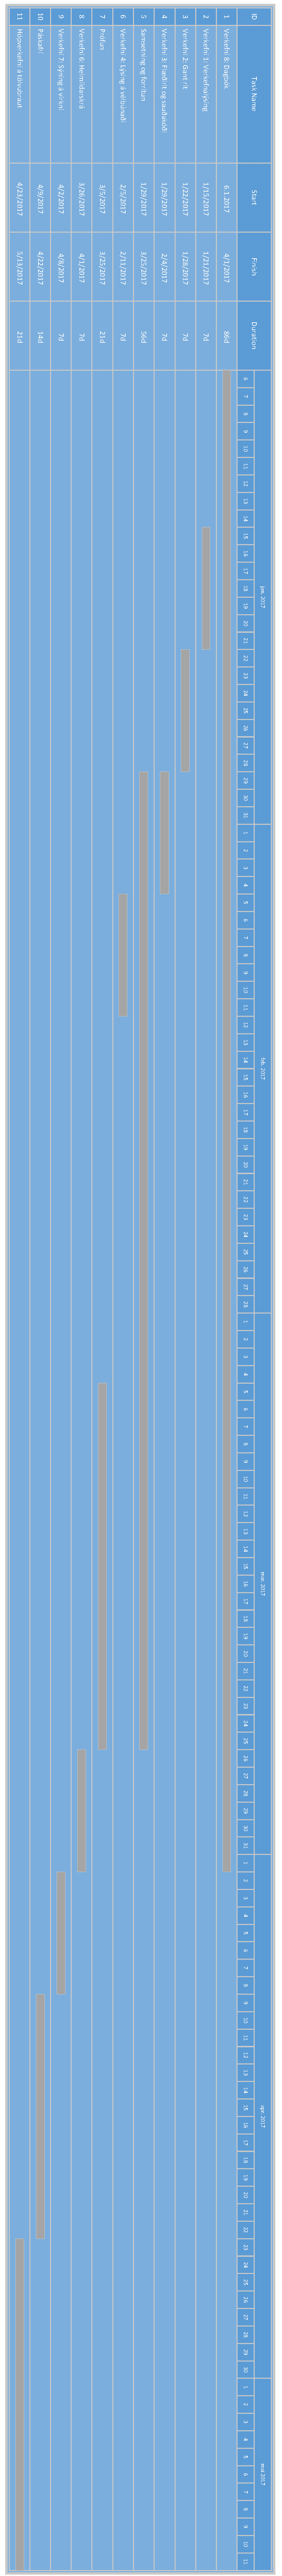
\includegraphics[scale=.16]{img/gant_rit}
\end{figure}
\newpage
\section{Flæðirit og sauðakóði}Það er ekki mikið af kóða sem þarf fyrir þetta verkefni. Flæðiritið mun verða fyrir notkun á vélinni.
\begin{figure}[h]
\includegraphics[scale=.6]{img/Retropie_portable_usage_flowchart}
\end{figure}

\section{Prófanir}
Hér skal gera lýsingu á prófunum á kerfinu . Til dæmis ef þið eruð með Arduino sem vefþjónn sem byrtir gildi frá hitamæli, rakamæli og gas mæli þá gæti prófunin verið svona: 1. prófun á vef, 2. prófun á hitamæli, .prófun á gasmæli hvert og eitt prófað sér áður en allt er sett saman og þá er gerð prófun á öllu kerfinu

Því miður fór eitthvað úrskeiðis í sendingu á pörtum til landsins, og við höfðum ekki tíma til þess að setja verkefnið saman. Við höfðum aftur á móti tíma til þess að setja upp allan hugbúnað sem þurfti fyrir verkefnið. Guðni gerði það að mestu leyti.

Ég setti upp mína eigin raspberry pi með retropie stýrikerfinu fyrst. Það tók tæpa 13 klukkutíma að downloada og installa öllum mismunandi pökkunum. Mest gerðist á sjálfu sér, en eitthvað fór úrskeiðis, og ég þurfti að fara gegnum allt til að finna hvaða pakka það vantaði (það var VLC). Eftir að allt var komið í gang þurfti ég bara að image-a sd kortið, og þá var allt tilbúið hugbúnaðarmegin.

Ég er líka að búa til tölvuleik fyrir annan áfanga í python og forritaði inn í hann stuðning fyrir leikjafjarstýringar og setti hann inn á pi-ið.
\section{Lokaorð}
Hér skal skrifa lokaorð um verkefnið, hvernig gékk, var gaman að vinna það hvað gékk vel og hvað illa. Hvernig var samvinnan :-) \cite{brock}

Því miður gekk verkefnið ekki alveg nógu vel vegna þess að við höfðum ekki alla partanna sem þurfti. Ég er viss um að ef við höfðum haft partana þá hefði allt gengið upp. Það sem við náðum að gera var nánast eingöngu hugbúnaðarmegin, stýrikerfi, tölvuleikir og þannig. Það gekk samt allt saman vel fyrir sig og við vorum snöggir að.
\newpage
\input{references}
\bibliographystyle{plain}
\bibliography{mybib}
\newpage
\section{Viðauki}
Hér skal vera dagbók frá öllum í verkefninu .
\begingroup
\obeylines
\input{dagbok.txt}
\endgroup
\subsection{Kóði Arduino}
Hér hef ég includað kóðan frá arduino sem er forritunarmálið C. Þetta getið þið endurtekið fyrir php kóða sem þið vistið í möppuni php eða python í möppunni python
\begingroup
\inputminted{python}{code/test.py}
\endgroup

\end{document}